\documentclass[unicode,11pt,a4paper,oneside,numbers=endperiod,openany]{scrartcl}
\usepackage[backend=biber, style=numeric, sorting=none]{biblatex}

\usepackage{ifthen}
\usepackage[utf8]{inputenc}
\usepackage{graphics}
\usepackage{graphicx}
\usepackage{hyperref}

\pagestyle{plain}
\voffset -5mm
\oddsidemargin  0mm
\evensidemargin -11mm
\marginparwidth 2cm
\marginparsep 0pt
\topmargin 0mm
\headheight 0pt
\headsep 0pt
\topskip 0pt        
\textheight 255mm
\textwidth 165mm

\newcommand{\duedate} {}
\newcommand{\setduedate}[1]{%
\renewcommand\duedate {See iCorsi for due date}}
\newcommand\isassignment {false}
\newcommand{\setassignment}{\renewcommand\isassignment {true}}
\newcommand{\ifassignment}[1]{\ifthenelse{\boolean{\isassignment}}{#1}{}}
\newcommand{\ifnotassignment}[1]{\ifthenelse{\boolean{\isassignment}}{}{#1}}

\newcommand{\assignmentpolicy}{
\begin{table}[h]
\begin{center}
\scalebox{0.8} {%
\begin{tabular}{|p{0.02cm}p{16cm}|}
\hline
&\\
\multicolumn{2}{|c|}{\Large\textbf{HPC Lab ---  Submission Instructions}}\\
\multicolumn{2}{|c|}{\large\textbf{(Please, notice that following instructions are mandatory: }}\\
\multicolumn{2}{|c|}{\large\textbf{submissions that don't comply with, won't be considered)}}\\
&\\
\textbullet & Assignments must be submitted to \href{https://www.icorsi.ch}{iCorsi} (i.e. in electronic format).\\
\textbullet & Provide both executable package and sources (e.g. C/C++ files, Matlab). 
If you are using libraries, please add them in the file. Sources must be organized in directories called:\\
\multicolumn{2}{|c|}{\textit{Project\_number\_lastname\_firstname}}\\
& and  the  file must be called:\\
\multicolumn{2}{|c|}{\textit{project\_number\_lastname\_firstname.zip}}\\
\multicolumn{2}{|c|}{\textit{project\_number\_lastname\_firstname.pdf}}\\
\textbullet &  The TAs will grade your project by reviewing your project write-up, and looking at the implementation 
                 you attempted, and benchmarking your code's performance.\\

\textbullet & You are allowed to discuss all questions with anyone you like; however: (i) your submission must list anyone you discussed problems with and (ii) you must write up your submission independently.\\
\hline
\end{tabular}
}
\end{center}
\end{table}
}
\newcommand{\punkte}[1]{\hspace{1ex}\emph{\mdseries\hfill(#1~\ifcase#1{Points}\or{Points}\else{Points}\fi)}}


\newcommand\serieheader[6]{
\thispagestyle{empty}%
\begin{flushleft}

\includegraphics[width=0.4\textwidth]{usi_inf.png}
\end{flushleft}
  \noindent%
  {\large\ignorespaces{\textbf{#1}}\hspace{\fill}\ignorespaces{ \textbf{#2}}}\\ \\%
  {\large\ignorespaces #3 \hspace{\fill}\ignorespaces #4}\\
  \noindent%
  \bigskip
  \hrule\par\bigskip\noindent%
  \bigskip {\ignorespaces {\Large{\textbf{#5}}}
  \hspace{\fill}\ignorespaces \large \ifthenelse{\boolean{\isassignment}}{\duedate}{#6}}
  \hrule\par\bigskip\noindent%  \linebreak
 }

\makeatletter
\def\enumerateMod{\ifnum \@enumdepth >3 \@toodeep\else
      \advance\@enumdepth \@ne
      \edef\@enumctr{enum\romannumeral\the\@enumdepth}\list
      {\csname label\@enumctr\endcsname}{\usecounter
        {\@enumctr}%%%? the following differs from "enumerate"
	\topsep0pt%
	\partopsep0pt%
	\itemsep0pt%
	\def\makelabel##1{\hss\llap{##1}}}\fi}
\let\endenumerateMod =\endlist
\makeatother




\usepackage{textcomp}





\usepackage{amsmath} 
\usepackage{amsfonts}
\usepackage{graphicx}
\usepackage{enumitem} 
\usepackage{longtable}
\usepackage{array}
\usepackage{xcolor}
\usepackage{booktabs}
\usepackage{multirow}
\usepackage{geometry}
\usepackage{listings}
\geometry{a4paper, margin=1in}
\lstdefinestyle{mystyle}{
    basicstyle=\ttfamily\small,
    keywordstyle=\color{blue},
    commentstyle=\color{green},
    stringstyle=\color{red},
    numbers=left,
    numberstyle=\tiny,
    stepnumber=1,
    frame=single,
    breaklines=true,
    captionpos=b,
    tabsize=2
}

\lstdefinelanguage{MyC++}{
    language=C++,
    morekeywords={std, vector, string},
}

\lstdefinelanguage{MyPython}{
    language=Python,
    morekeywords={self},
}

\lstdefinelanguage{MyBatch}{
    morekeywords={echo, pause, set},
    sensitive=false, 
    morecomment=[l]{REM}, 
    morestring=[b]",
}

\lstdefinelanguage{MyBash}{
    basicstyle=\ttfamily,
    breaklines=true,
    frame=single,
    keywordstyle=\color{blue},
    commentstyle=\color{gray},
    showstringspaces=false
}
\addbibresource{references.bib}

\begin{document}


\setassignment

\serieheader{High-Performance Computing Lab}{Institute of Computing}{Student: Zitian Wang}{Discussed with: None}{Solution for Project 2}{}
\newline

\assignmentpolicy
This project will introduce you to parallel programming using OpenMP. 

\section{Parallel reduction operations using OpenMP \punkte{20}}
\subsection{Dot Product}
\subsubsection{Two parallel versions of the dot product}
The \emph{reduction} clause automatically handles thread-local partial results and merges them at the end of the parallel section to produce the final outcome
\begin{lstlisting}[language=MyC++, style=mystyle, caption={Reduction pragma}]
void dot_product_reduction(double* a, double* b, long double& result){
#pragma omp parallel for reduction(+:alpha)
for (int i = 0; i < N; i++) {
    alpha += a[i] * b[i];
    }
}
\end{lstlisting}
The \emph{critical} instruction ensures that updating the shared variable alpha is performed serially, specifically during the summation phase, while the parallel section is responsible for calculating individual results, which involves the multiplication step.
\begin{lstlisting}[language=MyC++, style=mystyle, caption={Critical pragma}]
void dot_product_critical(double* a, double* b, long double& result, int N) {
    long double local_result = 0.0;

    #pragma omp parallel private(local_result)
    {
        local_result = 0.0;
        
        #pragma omp for
        for (int i = 0; i < N; i++) {
            local_result += a[i] * b[i];
        }

        #pragma omp critical
        {
            result += local_result;
        }
    }
}
\end{lstlisting}
\subsubsection{Strong scaling analysis}

To batch execute experiments with varying numbers of threads and different vector lengths, an execution script needs to be designed.

\begin{lstlisting}[language=MyBash, style=mystyle, caption={Bash Script for Dot Product Experiment}]
#!/bin/bash
VECTOR_LENGTHS=(100000 1000000 10000000 100000000 1000000000)
THREAD_COUNTS=(1 2 4 8 16 20)
g++ -O3 -fopenmp dotProduct.cpp -o dotProduct
if [ $? -ne 0 ]; then
    echo "Compilation failed!"
    exit 1
fi
for N in "${VECTOR_LENGTHS[@]}"; do
    
    FILENAME="experiment_results_${N}.csv"
    echo "Thread_Count,Method,Execution_Time" > $FILENAME
    for T in "${THREAD_COUNTS[@]}"; do
        export OMP_NUM_THREADS=$T
        echo "Running with Vector Length = $N and Threads = $T"

        ./dotProduct $N $T

        if [ $? -ne 0 ]; then
            echo "Execution failed for Vector Length = $N and Threads = $T!"
            exit 1
        fi
    done
done
echo "All experiments completed successfully."
\end{lstlisting}
After running the script, three key metrics, Serial Time, Reduction Time, and Critical Time will be obtained. 


\begin{table}[ht]
    \centering
    \caption{Execution Times (in seconds) for Different Vector Lengths and Thread Counts}
    \begin{tabular}{@{}cccccc@{}}
        \toprule
        \textbf{Vector Length} & \textbf{Threads} & \textbf{Serial Time} & \textbf{Reduction Time} & \textbf{Critical Time} \\ \midrule
        \multirow{6}{*}{100,000} 
        & 1  & 0.0471 & 0.0118 & 0.0118 \\
        & 2  & 0.0471 & 0.0061 & 0.0061 \\
        & 4  & 0.0472 & 0.0034 & 0.0034 \\
        & 8  & 0.0471 & 0.0025 & 0.0024 \\
        & 16 & 0.0472 & 0.0028 & 0.0027 \\
        & 20 & 0.0471 & 0.0040 & 0.0030 \\
        \midrule
        \multirow{6}{*}{1,000,000} 
        & 1  & 0.4716 & 0.1171 & 0.1175 \\
        & 2  & 0.4710 & 0.0589 & 0.0587 \\
        & 4  & 0.4713 & 0.0300 & 0.0297 \\
        & 8  & 0.4714 & 0.0159 & 0.0156 \\
        & 16 & 0.4710 & 0.0105 & 0.0093 \\
        & 20 & 0.4710 & 0.0090 & 0.0084 \\
        \midrule
        \multirow{6}{*}{10,000,000} 
        & 1  & 4.7752 & 1.3626 & 1.3630 \\
        & 2  & 4.7728 & 0.6993 & 0.6985 \\
        & 4  & 4.7756 & 0.6442 & 0.6440 \\
        & 8  & 4.7760 & 0.4832 & 0.5681 \\
        & 16 & 4.7826 & 0.5387 & 0.5407 \\
        & 20 & 4.7827 & 0.5254 & 0.6447 \\
        \midrule
        \multirow{6}{*}{100,000,000} 
        & 1  & 47.8156 & 13.6160 & 13.5554 \\
        & 2  & 47.8162 & 6.9151 & 6.9144 \\
        & 4  & 47.8293 & 6.2994 & 6.2982 \\
        & 8  & 47.7153 & 5.6159 & 5.6159 \\
        & 16 & 47.7149 & 4.4565 & 4.4643 \\
        & 20 & 47.7136 & 5.2087 & 5.2487 \\
        \midrule
        \multirow{6}{*}{1,000,000,000} 
        & 1  & 476.989 & 133.917 & 133.921 \\
        & 2  & 477.224 & 69.3902 & 69.4007 \\
        & 4  & 477.007 & 63.7676 & 63.7917 \\
        & 8  & 476.868 & 56.4091 & 56.4636 \\
        & 16 & 476.977 & 45.0795 & 44.9397 \\
        & 20 & 477.347 & 49.6325 & 49.7888 \\
        \bottomrule
    \end{tabular}
    \label{tab:experiment_times}
\end{table}
Based on the table, we can draw the following conclusions: the execution time of a serial program is linearly proportional to the vector length. The \texttt{critical} directive executes faster than the \texttt{reduction} clause, with this advantage becoming more pronounced as the vector length increases. The number of threads does not significantly impact the execution time of a serial program. While theoretically, increasing the number of threads should proportionally reduce the execution time for both the \texttt{critical} and \texttt{reduction} methods, the actual results show that the execution time for these two methods does not decrease by half when the number of threads increases from 8 to 16. Additionally, in some cases, the execution time increases when the number of threads reaches 20. This could be related to the fact that the CPU executing the program has only 20 cores.
The following graph is a figurative presentation of the above data, using logarithmic coordinates for ease of presentation.
\newpage
\begin{figure}[h]
    \centering
    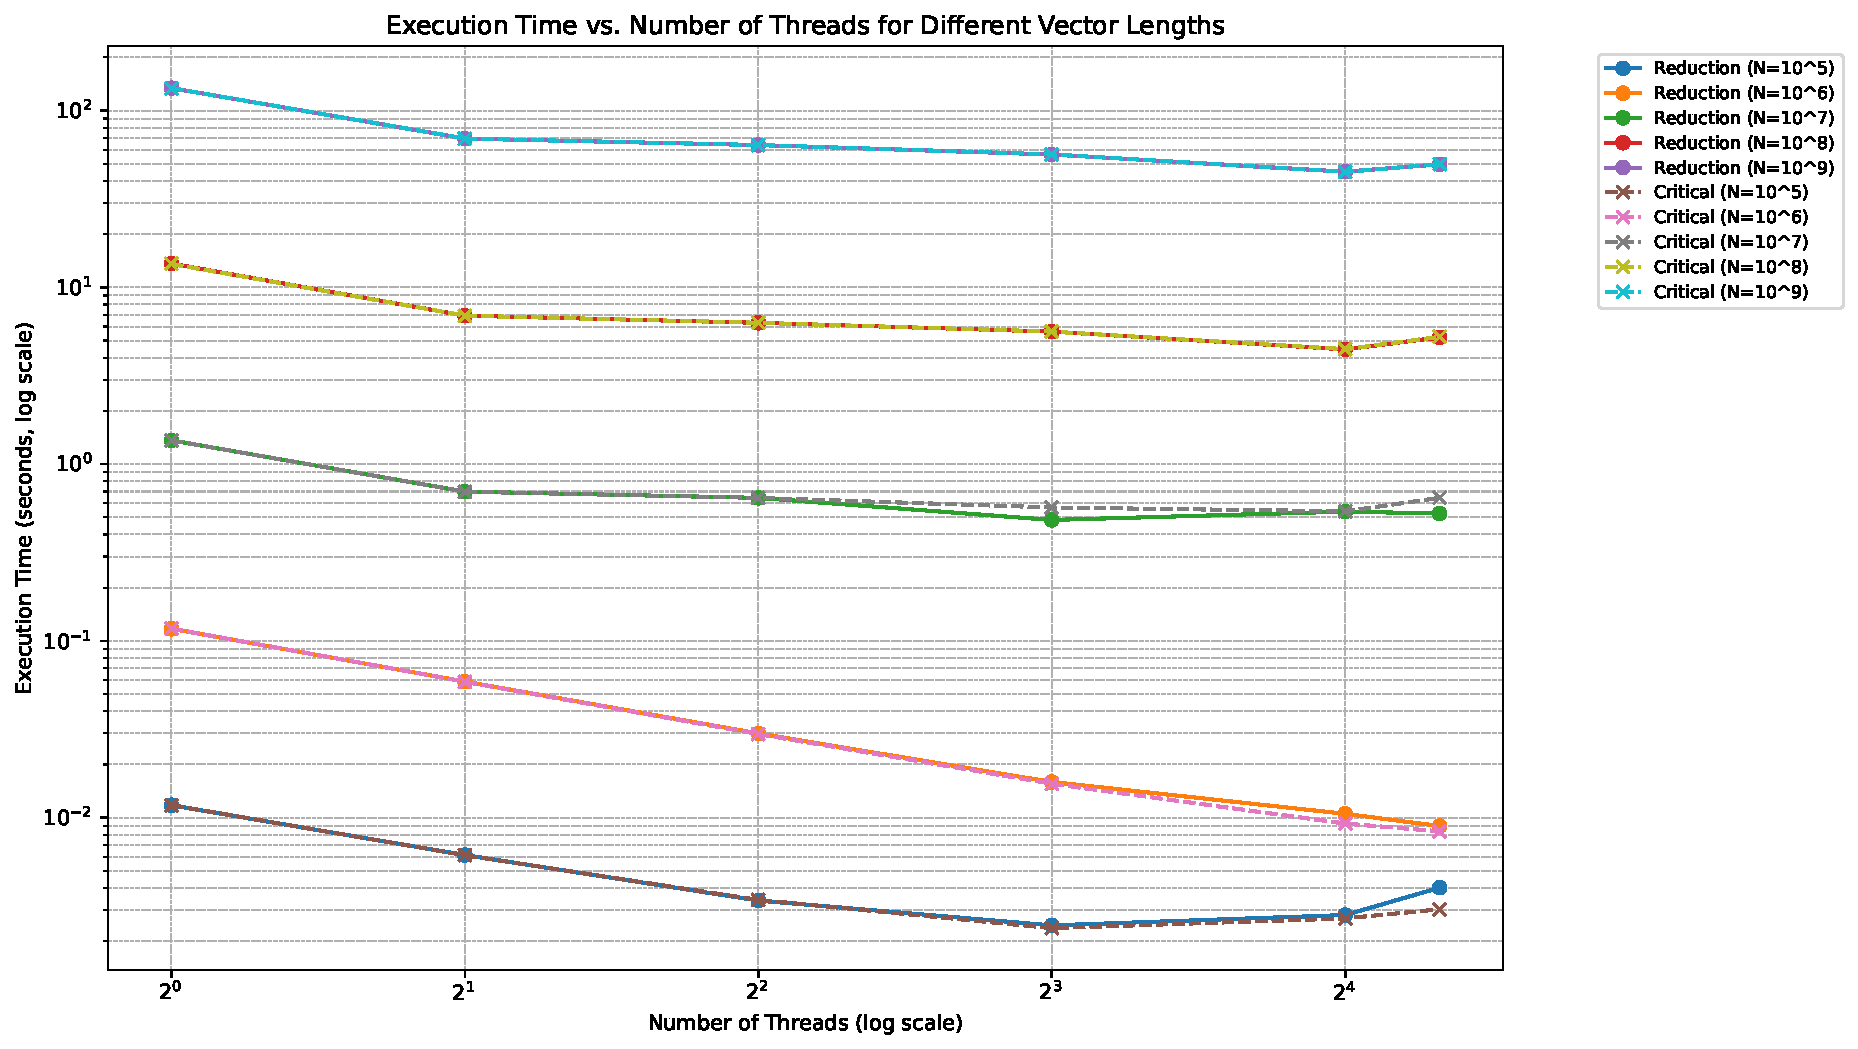
\includegraphics[width=1\textwidth]{pictures/execution_time_vs_threads.pdf}
    \caption{Execution time vs threads}
\end{figure}
\subsubsection{Analysis on the parallel efficiency}
In academic English, the definition of \textit{Parallel Efficiency} (Efficiency) can be expressed as follows:

\textit{Parallel Efficiency} (Efficiency) is defined as the ratio of speedup to the number of threads:

\[
\text{Efficiency} = \frac{\text{Speedup}}{\text{Number of Threads}}
\]

Where \textit{Speedup} is the ratio of serial execution time to parallel execution time:

\[
\text{Speedup} = \frac{T_{\text{serial}}}{T_{\text{parallel}}}
\]

Ideally, the closer the efficiency value is to 1, the better the parallelization performance\cite{hager2010introduction}. 
\begin{lstlisting}[language=MyPython, style=mystyle, caption={Plotting Parallel Efficiency for Reduction and Critical Methods}]
for vector_length in vector_lengths:
    serial_time = serial_times[vector_length]
    reduction_speedups = [serial_time / t for t in reduction_times[vector_length]]
    reduction_efficiency = [reduction_speedups[i] / threads[i] for i in range(len(threads))]
    plt.plot(threads, reduction_efficiency, label=f'Reduction (N=10^{int(np.log10(vector_length))})', marker='o')

for vector_length in vector_lengths:
    serial_time = serial_times[vector_length]
    critical_speedups = [serial_time / t for t in critical_times[vector_length]]
    critical_efficiency = [critical_speedups[i] / threads[i] for i in range(len(threads))]
    plt.plot(threads, critical_efficiency, label=f'Critical (N=10^{int(np.log10(vector_length))})', linestyle='--', marker='x')
\end{lstlisting}
The above code is used to calculate Efficiency when drawing a graph.
\begin{figure}[h]
    \centering
    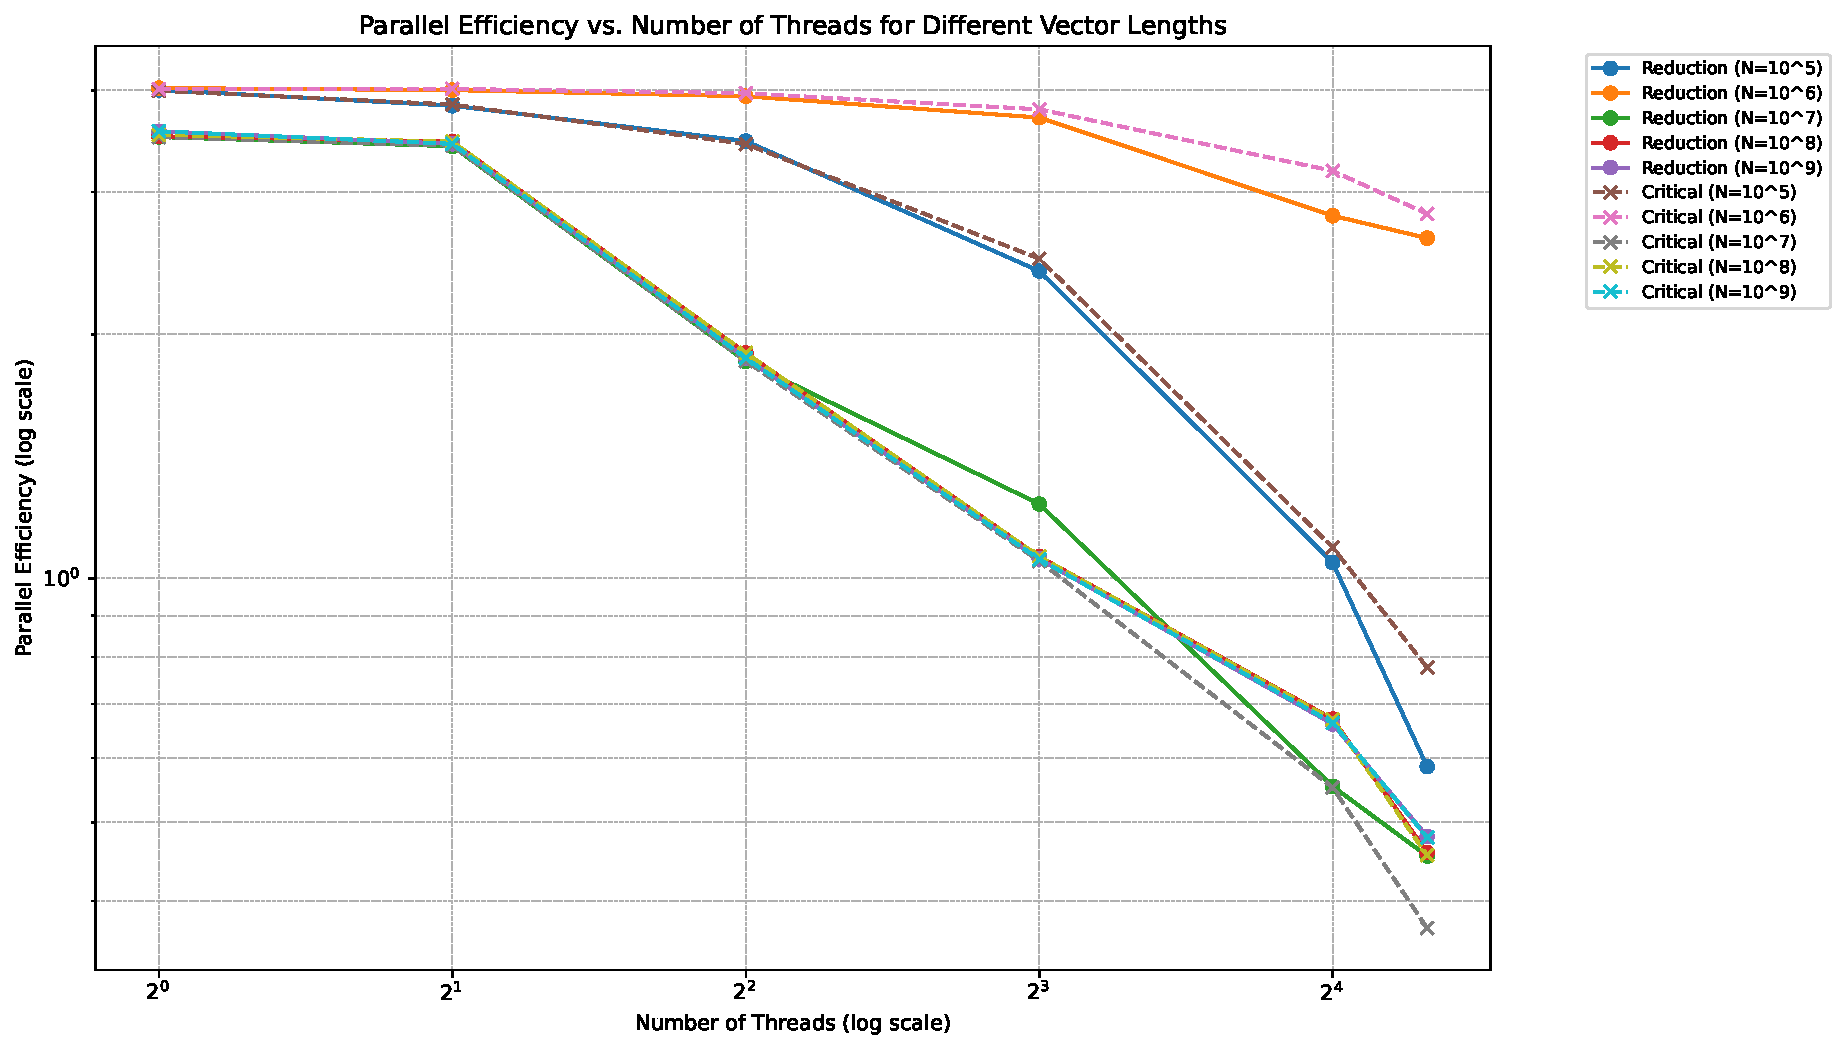
\includegraphics[width=1\textwidth]{pictures/parallel_efficiency_vs_threads.pdf}
    \caption{Parallel efficiency time vs threads}
\end{figure}

The graph with the logarithm of efficiency as the vertical axis more clearly illustrates the observations described in the previous question. By plotting the logarithm of efficiency, the deviations from ideal parallel performance become more apparent, especially as the number of threads increases beyond the optimal range, highlighting the diminishing returns in efficiency.

Initially, I used \texttt{\#pragma omp critical} within each loop iteration, which resulted in a very time-consuming process. Since then, I have modified the approach. Each thread now computes a partial dot product in the local variable \texttt{local\_result} and then accumulates it into the final result using \texttt{\#pragma omp critical}. By doing this, the critical section is executed only once after each thread completes its computation, significantly reducing the number of lock contentions and, consequently, the synchronization overhead. Therefore, in this exercise, the \textit{reduction} method demonstrates lower parallel efficiency compared to the \textit{critical} method.

Regarding the relationship between the number of threads, parallel efficiency, and workload size, both \textit{reduction} and \textit{critical} methods show significant efficiency improvements when the thread count is low. However, as the thread count increases to 16 or 20, the overhead from synchronization and scheduling begins to reduce efficiency. Larger vector lengths lead to higher parallel efficiency, particularly in multi-threaded scenarios, as the overhead between threads becomes relatively smaller, and the proportion of computation increases.

The benefits of multi-threading are evident when the vector length is large (e.g., \( N \geq 10^6 \)), where multi-threading achieves significant speedup. Conversely, for smaller vector lengths, using more threads yields diminishing returns or even inefficiencies due to synchronization overhead, making multi-threading less advisable for small-scale problems.
\newpage

\subsection{Approximating $\pi$}
\subsubsection{Serial and parallel versions method}

\begin{lstlisting}[language=MyC++, style=mystyle, caption={Serial Version of Computing Pi}]
/* TODO Serial Version of Computing Pi*/
time = omp_get_wtime();
sum = 0.0;
for (long int i = 0; i < N; i++) {
    double x = (i + 0.5) * dx;
    sum += 4.0 / (1.0 + x * x);
}
\end{lstlisting}

\begin{lstlisting}[language=MyC++, style=mystyle, caption={Parallel Version of Computing Pi}]
/* TODO Parallel Version of Computing Pi */
time = omp_get_wtime();
sum = 0.;
#pragma omp parallel for reduction(+:sum)
for (long int i = 0; i < N; i++) {
    double x = (i + 0.5) * dx;
    sum += 4.0 / (1.0 + x * x);
}
\end{lstlisting}
To parallelize the code, the \texttt{\#pragma omp parallel for reduction(+:sum)} directive is used because it automatically handles the local accumulation for each thread and then combines the results from all threads at the end. This approach significantly reduces the overhead of manually managing locks.

\subsubsection{Compare with parallel implementation and the serial version}\
\begin{lstlisting}[language=MyBash, style=mystyle, caption={Bash Script for Running Pi Program with OpenMP Support}]
#!/bin/bash
g++ -O3 -fopenmp pi.cpp -o pi
if [ $? -ne 0 ]; then
    echo "Compilation failed!"
    exit 1
fi
THREAD_COUNTS=(1 2 4 8)
for T in "${THREAD_COUNTS[@]}"; do
    export OMP_NUM_THREADS=$T
    echo "Running with $T thread(s):"
    ./pi
    if [ $? -ne 0 ]; then
    echo "Execution failed for $T thread(s)!"
    exit 1
    fi
    echo ""
done
echo "All experiments completed successfully."
\end{lstlisting}
    
\begin{table}[ht]
    \centering
    \caption{Serial and Parallel Execution Times for Approximating \( \pi \) with Different Thread Counts}
    \begin{tabular}{@{}cccccc@{}}
        \toprule
        \textbf{Threads} & \textbf{Serial Time (s)} & \textbf{Parallel Time (s)} & \textbf{Speedup} \\
        \midrule
        1 & 53.9293 & 53.9290 & 1.00 \\
        2 & 53.9291 & 27.0123 & 2.00 \\
        4 & 53.9331 & 13.5054 & 3.99 \\
        8 & 53.9288 & 6.7539  & 7.98 \\
        \bottomrule
    \end{tabular}
    \label{tab:pi_approximation_results}
\end{table}

\begin{figure}[h]
    \centering
    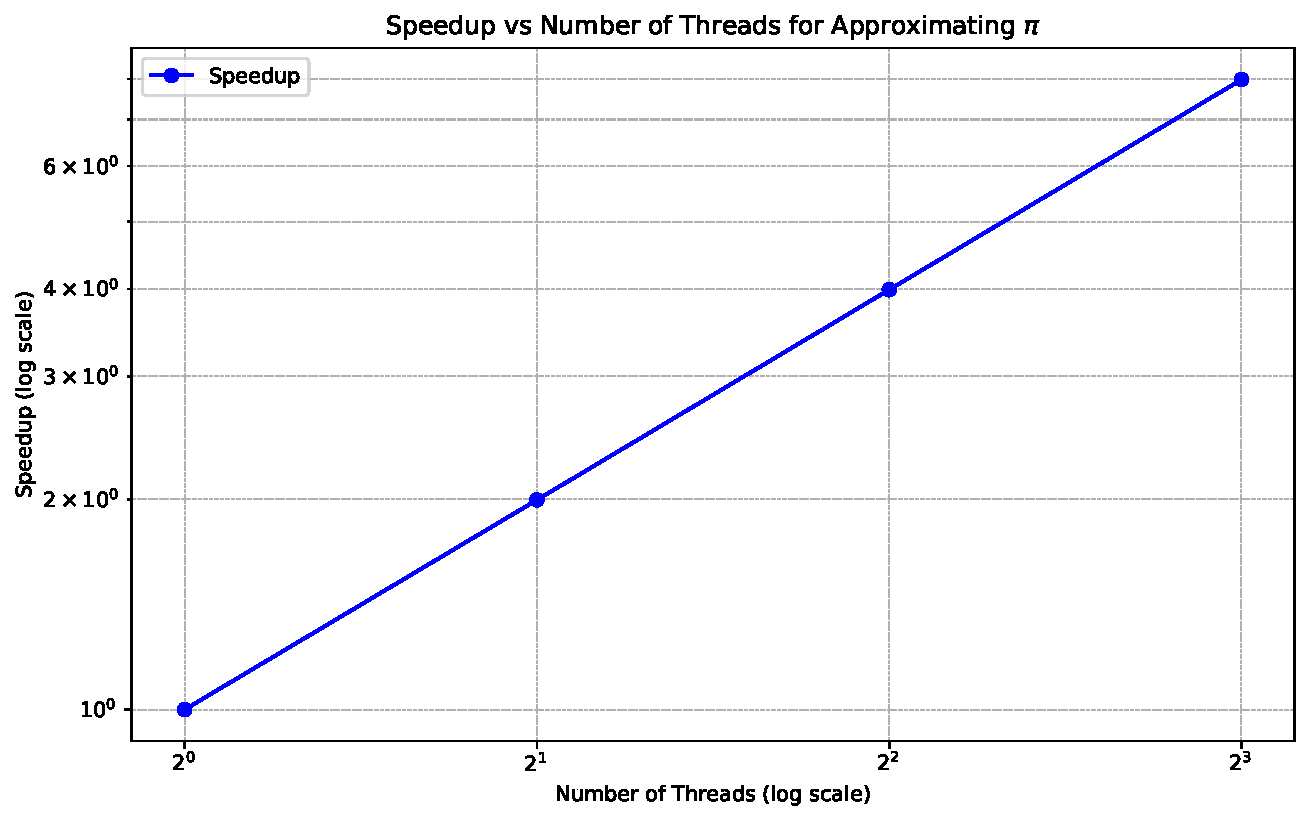
\includegraphics[width=1\textwidth]{pictures/pi_speedup_plot.pdf}
    \caption{Pi speedup}
\end{figure}

The plot generated from the experimental data reveals a diagonal line trending upwards, indicating that the speedup increases nearly linearly with the number of threads. This represents an ideal scenario, where parallel efficiency approaches 1. However, in many real-world situations (as discussed in the previous problem), achieving linear speedup becomes increasingly difficult as the number of threads grows. This is because managing threads introduces overheads associated with synchronization and communication, which tend to increase as the number of threads rises.

\section{The Mandelbrot set using OpenMP \punkte{20}}
\subsection{Computation kernel of the Mandelbrot set and number of iterations}
\begin{lstlisting}[language=MyC++, style=mystyle, caption={Mandelbrot Iteration Loop}]
while ((x2 + y2 <= 4.0) && (n < MAX_ITERS)) {
    y = 2 * x * y + cy;
    x = x2 - y2 + cx;
    x2 = x * x;
    y2 = y * y;
    n++;
    nTotalIterationsCount++;
}
\end{lstlisting}
\subsection{Parallelize the Mandelbrot code}
\begin{lstlisting}[language=MyC++, style=mystyle, caption={Parallel Mandelbrot Calculation with OpenMP}]
#pragma omp parallel for private(x, y, x2, y2, cx, cy) reduction(+:nTotalIterationsCount)
for (long j = 0; j < IMAGE_HEIGHT; j++) {
    cy = MIN_Y + j * fDeltaY;
    for (long i = 0; i < IMAGE_WIDTH; i++) {
        cx = MIN_X + i * fDeltaX;
        x = cx;
        y = cy;
        x2 = x * x;
        y2 = y * y;
        int n = 0;
        while ((x2 + y2 <= 4.0) && (n < MAX_ITERS)) {
            y = 2 * x * y + cy;
            x = x2 - y2 + cx;
            x2 = x * x;
            y2 = y * y;
            n++;
            nTotalIterationsCount++;
        }

        int c = ((long)n * 255) / MAX_ITERS;
        #pragma omp critical
        png_plot(pPng, i, j, c, c, c);
    }
}
\end{lstlisting}
\begin{table}[ht]
    \centering
    \caption{Benchmark Results for Serial and Parallel Mandelbrot Set Computation}
    \begin{tabular}{@{}ccccccc@{}}
        \toprule
        \textbf{Threads} & \textbf{Serial Time (s)} & \textbf{Parallel Time (s)} & \textbf{Speedup} & \textbf{Iterations/Second} & \textbf{MFlop/s} \\
        \midrule
        1  & 156.967 & 314.236 & 0.500 & $2.06 \times 10^8$ & 1648.12 \\
        2  & 156.970 & 235.837 & 0.666 & $2.74 \times 10^8$ & 2194.17 \\
        4  & 156.962 & 233.083 & 0.673 & $2.78 \times 10^8$ & 2220.10 \\
        8  & 156.968 & 208.487 & 0.753 & $3.10 \times 10^8$ & 2482.00 \\
        16 & 156.963 & 186.563 & 0.841 & $3.47 \times 10^8$ & 2773.68 \\
        20 & 156.979 & 181.296 & 0.866 & $3.57 \times 10^8$ & 2854.26 \\
        \bottomrule
    \end{tabular}
    \label{tab:mandelbrot_results}
\end{table}
\begin{figure}[h]
    \centering
    
\includegraphics[width=0.45\textwidth]{pictures/mandel.png}
    \caption{The Mandelbrot set}
\end{figure}
\begin{figure}[h]
    \centering
    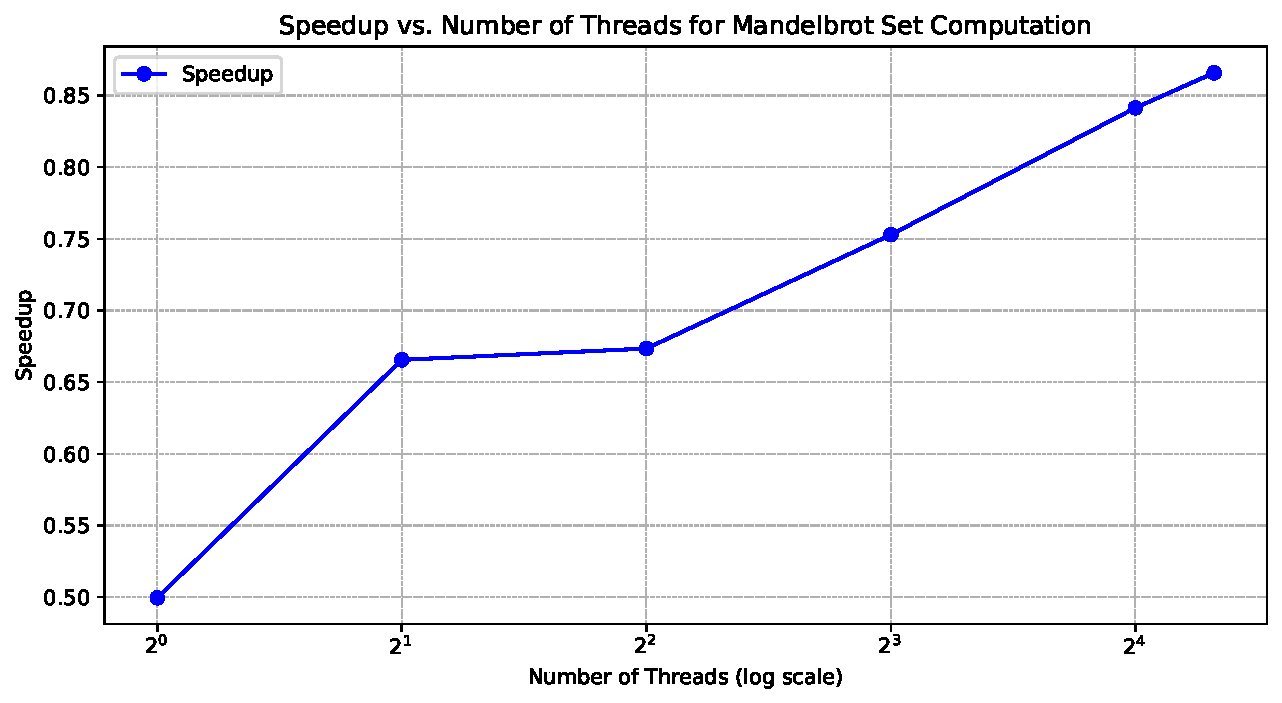
\includegraphics[width=1\textwidth]{pictures/speedup_plot.pdf}
    \caption{Speedup}
\end{figure}
The speedup shows little improvement when the number of threads increases from 2 to 4, likely due to the computational nature of the Mandelbrot set, which varies in complexity across different regions of the complex plane. Some regions require more iterations to determine whether they belong to the Mandelbrot set, while others require fewer iterations. This variation can cause an imbalance in workload distribution among the threads, with some handling more complex regions and others dealing with simpler regions. As a result, some threads may finish earlier, leading to increased waiting time for the remaining threads, thereby affecting overall parallel efficiency. However, as the number of threads increases to 8, 16, or even 20, the speedup begins to grow more linearly. This is likely because each thread handles a smaller workload, resulting in more efficient task processing.

\section{Bug hunt \punkte{15}}
\paragraph{bug1}
The \texttt{tid} is used to print the thread number, but due to the nesting of the \texttt{\{\}} block and the inner \texttt{for} loop, the \texttt{tid} may not be unique within the loop, potentially causing confusion regarding thread numbers. To resolve this, move the \texttt{tid} fetching operation inside the \texttt{for} loop body so that the current thread's number is fetched again each time the loop iterates, ensuring the uniqueness of the thread identifier.
\paragraph{bug2}
The variable \texttt{total} is declared and used in the parallel region, but it is shared among threads, causing data contention as each thread attempts to modify it. This issue can be resolved by utilizing OpenMP's \texttt{reduction(+:total)} mechanism, which converts \texttt{total} into a local cumulative variable for each thread. After all threads complete their calculations, the \texttt{reduction} directive combines the individual \texttt{total} values, ensuring accurate final results without data contention.
\paragraph{bug3}
The \texttt{\#pragma omp barrier} cannot be used within a \texttt{section} structure inside a parallel region because it can lead to a deadlock. This occurs when some threads are still executing sections while others reach the barrier, causing all threads to wait indefinitely for one another, halting execution. To prevent such mis-synchronization and avoid potential deadlocks, remove the \texttt{\#pragma omp barrier} from the \texttt{print\_results()} function.
\paragraph{bug4}
For an array \texttt{a} of size \( N \times N \), where \( N = 1048 \), each thread needs to allocate a large chunk of memory for its own copy. This can exceed the available stack space, leading to a segmentation fault. To resolve this issue, the stack size for all additional threads can be adjusted via the environment variable \texttt{OMP\_STACKSIZE}, which allows for controlling and increasing the stack size limit to prevent such errors.
\paragraph{bug5}
In the code, the two \texttt{\#pragma omp sections} are executed by different threads, both of which involve two locks: \texttt{locka} and \texttt{lockb}. If the threads execute simultaneously, with one thread holding \texttt{locka} and the other holding \texttt{lockb}, they can end up waiting for each other to release their respective locks, resulting in a deadlock. To prevent deadlocks, ensure that both threads acquire the locks in the same order. This way, both threads will follow a consistent locking sequence, avoiding situations where one thread waits indefinitely for the other.
\section{Parallel histogram calculation using OpenMP \punkte{15}}
\begin{lstlisting}[language=MyC++, style=mystyle, caption={Parallel Histogram Calculation with OpenMP}]
time_start = walltime();
long local_histograms[BINS * omp_get_max_threads()] = {0};

#pragma omp parallel shared(local_histograms)
{
    int tid = omp_get_thread_num();
    long* local_hist = &local_histograms[tid * BINS];

    #pragma omp for
    for (long i = 0; i < VEC_SIZE; ++i) {
        dist[vec[i]]++;
    }
}
\end{lstlisting}
\begin{table}[h]
    \centering
    \caption{Strong Scaling Results for Histogram Calculation}
    \begin{tabular}{lccc}
        \toprule
        \textbf{Number of Threads} & \textbf{Parallel Time (s)} & \textbf{Serial Time (s)} & \textbf{Speedup} \\ \midrule
        1   & 1.85422   & 1.85422   & 1.00 \\ 
        2   & 1.58072   & 1.85422   & 1.17 \\ 
        4   & 1.01373   & 1.85422   & 1.83 \\ 
        8   & 0.840241  & 1.85422   & 2.21 \\ 
        16  & 0.831195  & 1.85422   & 2.23 \\ 
        32  & 0.81123   & 1.85422   & 2.29 \\ 
        64  & 0.80345   & 1.85422   & 2.31 \\ 
        128 & 0.79932   & 1.85422   & 2.32 \\ \bottomrule
    \end{tabular}
    \label{tab:strong_scaling}
\end{table}
\begin{figure}[h]
    \centering
    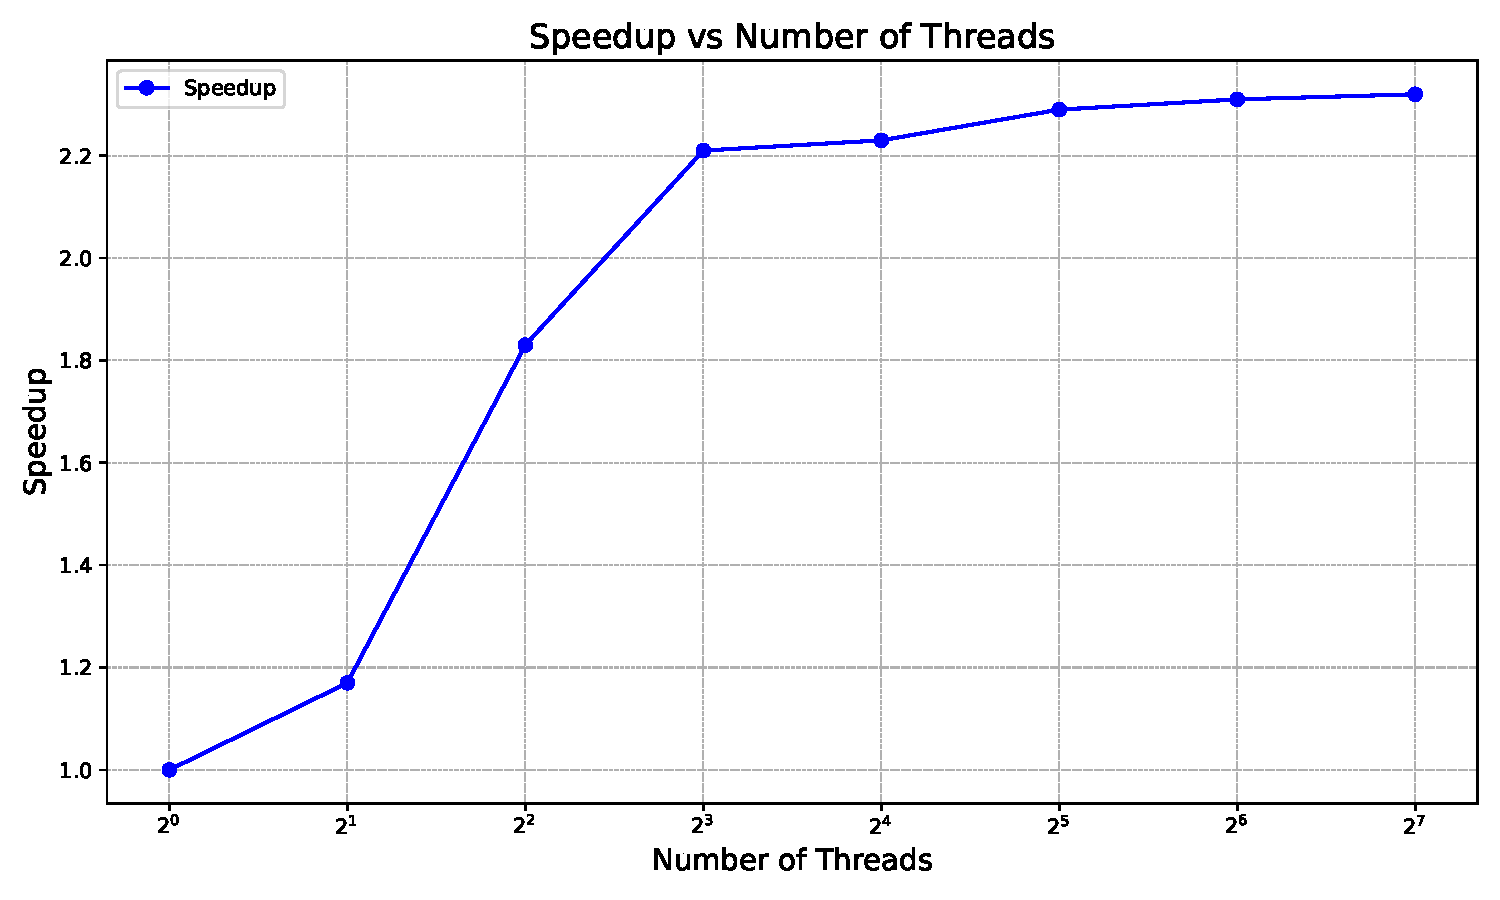
\includegraphics[width=1\textwidth]{pictures/histogram_speedup_plot.pdf}
    \caption{Histogram speedup}
\end{figure}
In line with the previous conclusion, the marginal benefit of performance improvement decreases significantly once the number of threads exceeds 8. Beyond this point, additional threads provide diminishing returns in terms of speedup, likely due to increased overhead from thread management, synchronization, and reduced workload per thread. In particular, the performance gain from increasing the number of threads from 1 to 2 is not significant, likely because the synchronization overhead between threads constitutes a larger percentage of the total runtime, especially when updating the histogram. It is only when the number of threads reaches a certain threshold that the computational benefits begin to outweigh the synchronization costs, leading to more noticeable performance improvements.


\section{Parallel loop dependencies with OpenMP \punkte{15}}
\begin{lstlisting}[language=MyC++, style=mystyle, caption={loop parallelization}]
#pragma omp parallel for firstprivate(Sn) lastprivate(Sn)
for (n = 0; n <= N; ++n) {
    opt[n] = Sn;
    Sn *= up;
}
\end{lstlisting}
\texttt{firstprivate(Sn)} ensures that each thread starts with the initial value of \texttt{Sn} from the serial portion when entering the parallel region, guaranteeing consistent initial states for all threads, while \texttt{lastprivate(Sn)} ensures that the value of \texttt{Sn} from the last iteration is saved back to the serial portion after the parallel region.
\begin{lstlisting}[language=MyC++, style=mystyle, caption={reduction}]
#pragma omp parallel for reduction(+:temp)
for (n = 0; n <= N; ++n) {
    temp += opt[n] * opt[n];
}
\end{lstlisting}
Since all threads need to accumulate the value of \texttt{temp}, the \texttt{reduction(+:temp)} clause is used, which allows for safe accumulation in a parallel environment and ultimately combines the partial sums from each thread.

\begin{table}[h]
    \centering
    \caption{Comparison of Sequential and Parallel Execution for Recursion Problem}
    \begin{tabular}{lcc}
        \toprule
        \textbf{Metric} & \textbf{Sequential} & \textbf{Parallel (OMP)} \\ \midrule
        RunTime (s) & 6.736231 & 0.410847 \\
        Final Result $S_n$ & 485165097.62511122 & 2.7182818255291776 \\
        Result $||opt||^2_2$ & $5.8846 \times 10^{15}$ & 3.194528 \\ \bottomrule
    \end{tabular}
    \label{tab:recur_comparison}
\end{table}

    

\printbibliography
\end{document}